\chapter{Limas dan Kerucut}\label{ch:g8:solids}

Sesudah \omterm{def:g7:areas:prism}{prisma} dan \omterm{def:g7:areas:prism}{tabung} pada \cref{ch:g7:areas} --- yaitu \omterm{def:g5:solids:def}{bangun
ruang} yang penampangnya tetap --- datanglah \omterm{def:g5:solids:def}{bangun ruang} yang punya
titik puncak: \omterm{def:g8:solids:def}{limas} dan \omterm{def:g8:solids:def}{kerucut}. Rumus \omterm{def:g6:measure:volume}{volumenya} membawa faktor
terkenal $\frac13$, yang dibuat masuk akal lalu dipakai pada bab ini;
kajian \omterm{def:g5:solids:def}{bangun ruang} berlanjut dengan bola dan irisan pada
\cref{ch:g9:solids}.

\section{Menguraikan limas dan kerucut}

\begin{definition}[Limas, kerucut]\label{def:g8:solids:def}
\begin{itemize}
  \item \emph{Limas}\index{limas} punya \omterm{def:g4:geometry:polygon}{segi banyak} sebagai
        \emph{alasnya} dan sebuah titik, yaitu \emph{puncaknya}, yang
        dihubungkan ke tiap \omterm{def:g5:solids:def}{titik sudut} alasnya oleh sisi berbentuk
        segitiga. \emph{Tingginya} adalah jarak dari puncaknya ke
        bidang alasnya.
  \item \emph{Kerucut}\index{kerucut} adalah bangun yang dibangun
        dengan cara yang sama di atas cakram: alas berbentuk cakram,
        sebuah puncak, dan selimut lengkung.
\end{itemize}
Sebuah limas disebut \emph{beraturan} ketika alasnya \omterm{def:g4:geometry:polygon}{segi banyak}
beraturan (persegi, \omterm{def:g6:shapes:triangles}{segitiga sama sisi}, \dots) dan puncaknya duduk
\omterm{def:g6:lines:perp}{tegak lurus} di atas pusat alasnya.
\end{definition}

\begin{omfigure}
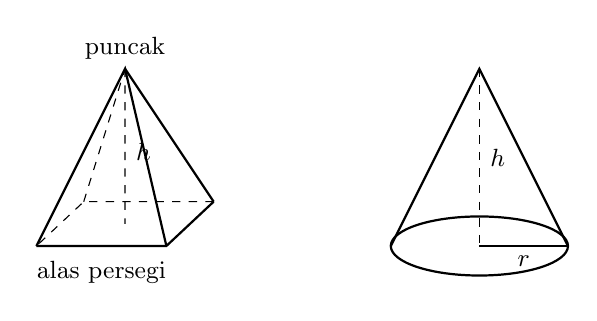
\begin{tikzpicture}[scale=0.75]
  % limas persegi
  \coordinate (P1) at (-1.3,0);
  \coordinate (P2) at (0.9,0);
  \coordinate (P3) at (1.7,0.75);
  \coordinate (P4) at (-0.5,0.75);
  \coordinate (S) at (0.2,3.0);
  \draw[thick] (P1) -- (P2) -- (P3);
  \draw[dashed] (P3) -- (P4) -- (P1);
  \draw[thick] (P1) -- (S) -- (P2);
  \draw[thick] (P3) -- (S);
  \draw[dashed] (P4) -- (S);
  \draw[dashed] (S) -- (0.2,0.375);
  \node[right, font=\small] at (0.22,1.6) {$h$};
  \node[above, font=\small] at (S) {puncak};
  \node[below, font=\small] at (-0.2,-0.1) {alas persegi};
  % kerucut
  \begin{scope}[xshift=6.2cm]
  \draw[thick] (0,0) ellipse (1.5 and 0.5);
  \coordinate (T) at (0,3.0);
  \draw[thick] (-1.5,0) -- (T) -- (1.5,0);
  \draw[dashed] (T) -- (0,0);
  \node[right, font=\small] at (0.02,1.5) {$h$};
  \draw[thin] (0,0) -- (1.5,0) node[midway, below, font=\small] {$r$};
  \end{scope}
\end{tikzpicture}

{\small Sebuah \omterm{def:g8:solids:def}{limas} beralas persegi dan sebuah \omterm{def:g8:solids:def}{kerucut}: satu alas
bersegi banyak atau berbentuk lingkaran, satu puncak, dan tinggi yang
diukur \omterm{def:g6:lines:perp}{tegak lurus} terhadap alasnya.}
\end{omfigure}

\begin{example}[Membilang sisi, rusuk, titik sudut]\label{ex:g8:solids:count}
\omterm{def:g8:solids:def}{Limas} beralas persegi punya $5$ sisi ($1$ persegi $+ 4$
segitiga), $8$ \omterm{def:g5:solids:def}{rusuk} dan $5$ \omterm{def:g5:solids:def}{titik sudut}. Dengan alas bersegi $n$:
$n + 1$ sisi, $2n$ \omterm{def:g5:solids:def}{rusuk}, $n + 1$ \omterm{def:g5:solids:def}{titik sudut}. Periksalah pola kecil
milik Euler: sisi $+$ \omterm{def:g5:solids:def}{titik sudut} $=$ \omterm{def:g5:solids:def}{rusuk} $+ 2$.
\end{example}

\section{Volume}

\begin{theorem}[Volume limas atau kerucut]\label{thm:g8:solids:volume}
Untuk \omterm{def:g8:solids:def}{limas} atau \omterm{def:g8:solids:def}{kerucut} dengan luas alas $B$ dan tinggi $h$:
\[
V = \frac{1}{3}\, B \times h
\]
--- yaitu sepertiga \omterm{def:g7:areas:prism}{prisma} atau \omterm{def:g7:areas:prism}{tabung} dengan alas dan tinggi yang
sama. Untuk \omterm{def:g8:solids:def}{kerucut} beralas \omterm{def:g3:shapes:shapes}{jari-jari} $r$: $V = \frac13 \pi r^2 h$.
\end{theorem}
\admitted

\begin{remark}[Mengapa sepertiga?]
Isilah \omterm{def:g8:solids:def}{limas} berongga dengan air lalu tuangkan ke dalam \omterm{def:g7:areas:prism}{prisma} dengan
alas dan tinggi yang sama: airnya pas tiga kali penuangan. Lebih baik
lagi: sebuah \omterm{def:g5:solids:def}{kubus} dapat dipotong menjadi tiga \omterm{def:g8:solids:def}{limas} yang identik,
masing-masing punya sebuah sisi kubusnya sebagai alas dan sebuah \omterm{def:g5:solids:def}{titik
sudut} kubusnya sebagai puncak (cobalah membayangkannya!). Bukti
umumnya memakai pengintegralan, alat di buku Sekolah Menengah.
\end{remark}

\begin{example}\label{ex:g8:solids:volume}
Sebuah \omterm{def:g8:solids:def}{limas} punya alas persegi bersisi $5$ cm dan tinggi $9$ cm:
\begin{enumerate}
  \item luas alasnya: $B = 5^2 = 25$ cm$^2$;
  \item \omterm{def:g6:measure:volume}{volumenya}: $V = \frac13 \times 25 \times 9 = 25 \times 3 = 75$
        cm$^3$.
\end{enumerate}
Sebuah \omterm{def:g8:solids:def}{kerucut} es krim berjari-jari $3$ cm dan tinggi $10$ cm:
\[
V = \frac13 \times \pi \times 3^2 \times 10 = 30\pi \approx 94
\text{ cm}^3 .
\]
\end{example}

\begin{example}[Hati-hati dengan tingginya]\label{ex:g8:solids:slant}
Untuk \omterm{def:g8:solids:def}{kerucut}, jangan mengacaukan tingginya $h$ (dari puncak ke pusat
alasnya, \omterm{def:g6:lines:perp}{tegak lurus}) dengan \emph{garis pelukisnya} $s$ (dari puncak
ke tepinya). Keduanya dihubungkan Pythagoras
(\cref{thm:g8:pythagoras:direct}) pada \omterm{def:g6:shapes:triangles}{segitiga siku-siku}
puncak--pusat--tepi:
\[
s^2 = h^2 + r^2 .
\]
Karena itu \omterm{def:g8:solids:def}{kerucut} dengan $r = 3$ dan $s = 5$ punya tinggi
$h = \sqrt{25 - 9} = 4$, dan \omterm{def:g6:measure:volume}{volume}
$\frac13 \pi \times 9 \times 4 = 12\pi$.
\end{example}

\begin{method}[Soal volume]\label{met:g8:solids:method}
\begin{enumerate}
  \item Kenalilah \omterm{def:g5:solids:def}{bangun ruangnya} (\omterm{def:g7:areas:prism}{prisma}/\omterm{def:g7:areas:prism}{tabung}: $V = Bh$;
        \omterm{def:g8:solids:def}{limas}/\omterm{def:g8:solids:def}{kerucut}: $V = \frac13 Bh$);
  \item hitunglah luas alasnya $B$ lebih dahulu, sebagai langkah yang
        terpisah;
  \item periksalah bahwa tingginya \omterm{def:g6:lines:perp}{tegak lurus} terhadap alasnya
        (pakailah Pythagoras kalau garis pelukisnya yang diberikan);
  \item kalikan, jagalah satuannya tetap serasi, lalu ubahlah pada
        akhirnya kalau perlu ($1$ L $= 1000$ cm$^3$).
\end{enumerate}
\end{method}

\section{Jaring-jaring}

\begin{example}[Jaring-jaring limas]\label{ex:g8:solids:net}
Membuka lipatan sebuah \omterm{def:g8:solids:def}{limas} beraturan beralas persegi memipihkannya
menjadi \emph{\omterm{def:g5:solids:net}{jaring-jaringnya}}: alas perseginya dengan empat \omterm{def:g6:shapes:triangles}{segitiga sama
kaki} yang identik menempel pada sisinya. Sisi segitiganya yang sama
panjang adalah \emph{\omterm{def:g5:solids:def}{rusuk} tegak} limasnya --- panjangnya bukan $h$
dan bukan pula tinggi sisi tegaknya, jadi berilah nama dengan hati-hati
sebelum memotong kartonnya.
\end{example}

\begin{omfigure}
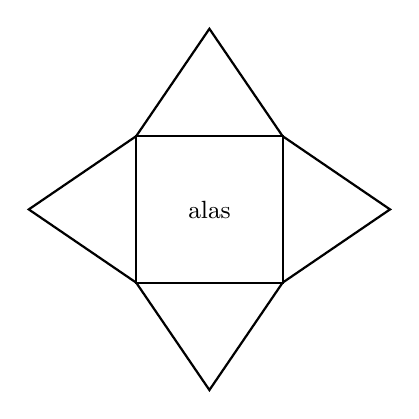
\begin{tikzpicture}[scale=0.62]
  \draw[thick] (0,0) rectangle (3,3);
  \draw[thick] (0,0) -- (1.5,-2.2) -- (3,0);
  \draw[thick] (3,0) -- (5.2,1.5) -- (3,3);
  \draw[thick] (0,3) -- (1.5,5.2) -- (3,3);
  \draw[thick] (0,0) -- (-2.2,1.5) -- (0,3);
  \node[font=\small] at (1.5,1.5) {alas};
\end{tikzpicture}

{\small \omterm{def:g5:solids:net}{Jaring-jaring} \omterm{def:g8:solids:def}{limas} beralas persegi: lipatlah keempat
segitiganya ke atas sampai puncaknya bertemu.}
\end{omfigure}

\section{Latihan}

\begin{exercise}[$\star$]\label{exo:g8:solids:1}
Berapa sisi, \omterm{def:g5:solids:def}{rusuk} dan \omterm{def:g5:solids:def}{titik sudut} yang dipunyai \omterm{def:g8:solids:def}{limas} beralas
segitiga (yaitu \emph{bidang empat})? Dengan alas bersegi enam?
\end{exercise}

\begin{exercise}[$\star$]\label{exo:g8:solids:2}
Hitunglah \omterm{def:g6:measure:volume}{volume} \omterm{def:g8:solids:def}{limas} dengan luas alas $36$ cm$^2$ dan tinggi
$10$ cm; lalu \omterm{def:g6:measure:volume}{volume} \omterm{def:g8:solids:def}{limas} dengan alas persegi panjang
$6 \times 4$ cm dan tinggi $7.5$ cm.
\end{exercise}

\begin{exercise}[$\star$]\label{exo:g8:solids:3}
Hitunglah \omterm{def:g6:measure:volume}{volume} \omterm{def:g8:solids:def}{kerucut} berjari-jari $5$ cm dan tinggi $9$ cm
(persis dengan $\pi$, lalu \omterm{def:g4:numbers:round}{dibulatkan} ke cm$^3$).
\end{exercise}

\begin{exercise}[$\star$]\label{exo:g8:solids:4}
Sebuah \omterm{def:g7:areas:prism}{tabung} dan sebuah \omterm{def:g8:solids:def}{kerucut} punya \omterm{def:g3:shapes:shapes}{jari-jari} yang sama $4$ cm dan
tinggi yang sama $12$ cm. Hitunglah kedua \omterm{def:g6:measure:volume}{volumenya}. Berapa
perbandingannya?
\end{exercise}

\begin{exercise}[$\star$]\label{exo:g8:solids:5}
Sebuah \omterm{def:g8:solids:def}{limas} punya \omterm{def:g6:measure:volume}{volume} $56$ cm$^3$ dan tinggi $8$ cm. Berapa luas
alasnya? (Tulislah rumus \omterm{def:g6:measure:volume}{volumenya} lalu selesaikan.)
\end{exercise}

\begin{exercise}[$\star$]\label{exo:g8:solids:6}
Sketsalah \omterm{def:g5:solids:net}{jaring-jaring} \omterm{def:g8:solids:def}{kerucut} (sebuah cakram untuk alasnya, dan
sebuah juring cakram yang lebih besar untuk selimutnya). Ukuran
\omterm{def:g8:solids:def}{kerucut} yang mana yang menjadi \omterm{def:g3:shapes:shapes}{jari-jari} juring itu: tingginya $h$
atau garis pelukisnya $s$?
\end{exercise}

\begin{exercise}[$\star\star$]\label{exo:g8:solids:7}
Piramida Louvre punya alas persegi bersisi kira-kira $35$ m dan
tinggi kira-kira $22$ m. Taksirlah \omterm{def:g6:measure:volume}{volumenya}, sampai ratusan meter
kubik terdekat.
\end{exercise}

\begin{exercise}[$\star\star$]\label{exo:g8:solids:8}
Sebuah \omterm{def:g8:solids:def}{kerucut} punya garis pelukis $13$ cm dan \omterm{def:g3:shapes:shapes}{jari-jari} alas $5$ cm.
Hitunglah tingginya, lalu \omterm{def:g6:measure:volume}{volumenya} (persis dengan $\pi$).
\end{exercise}

\begin{exercise}[$\star\star$]\label{exo:g8:solids:9}
Sebuah gelas berbentuk \omterm{def:g8:solids:def}{kerucut} berjari-jari $4$ cm dan tinggi $9$ cm
diisi sampai penuh, lalu dituangkan ke dalam gelas berbentuk \omterm{def:g7:areas:prism}{tabung}
berjari-jari $4$ cm. Tinggi berapa yang dicapai cairannya di dalam \omterm{def:g7:areas:prism}{tabungnya}?
\end{exercise}

\begin{exercise}[$\star\star$]\label{exo:g8:solids:10}
Sebuah jam pasir dibuat dari dua \omterm{def:g8:solids:def}{kerucut} yang identik (\omterm{def:g3:shapes:shapes}{jari-jari}
$2$ cm, tinggi $4.5$ cm) yang disambung pada puncaknya. Seluruh
pasirnya persis mengisi satu \omterm{def:g8:solids:def}{kerucut}. Hitunglah \omterm{def:g6:measure:volume}{volume} pasirnya
(persis, lalu dalam cm$^3$ yang \omterm{def:g4:numbers:round}{dibulatkan} ke persepuluhan), dan
berapa bagian dari \omterm{def:g6:measure:volume}{volume} dalam jam pasirnya yang ditempati pasirnya.
\end{exercise}

\begin{exercise}[$\star\star\star$]\label{exo:g8:solids:11}
Sebuah \omterm{def:g8:solids:def}{limas} beralas persegi dengan sisi alas $6$ cm punya puncaknya
tepat di atas sebuah pojok alasnya, pada tinggi $8$ cm.
\begin{enumerate}
  \item Apakah rumus $V = \frac13 Bh$ tetap berlaku? (Ya, memang ---
        puncaknya tidak harus berada di tengah. Hitunglah $V$.)
  \item Hitunglah panjang \omterm{def:g5:solids:def}{rusuk} tegak yang terpanjang, dari puncaknya
        ke pojok alasnya yang di seberang (dua langkah Pythagoras:
        diagonal alasnya lebih dahulu).
\end{enumerate}
\end{exercise}

\section{Soal: Kubus yang dipotong menjadi tiga limas}

\begin{problem}[{Soal akhir pekan --- dari mana faktor $\frac13$
datang, dan apa yang terjadi pada limas yang dipotong di setengah tingginya}]
\label{pb:g8:solids:1}
Catatan sesudah \cref{thm:g8:solids:volume} menyatakan bahwa sebuah
\omterm{def:g5:solids:def}{kubus} dapat dipotong menjadi tiga \omterm{def:g8:solids:def}{limas} yang identik --- ``cobalah
membayangkannya!''. Soal ini membayangkannya dengan tepat, memperoleh
faktor terkenal $\frac13$ darinya secara jujur, lalu memotong kubusnya
dengan cara kedua menjadi \emph{enam} \omterm{def:g8:solids:def}{limas}, dan berakhir dengan
mengiris sebuah \omterm{def:g8:solids:def}{limas} pada setengah tingginya --- dengan hasil yang
sedikit orang menebaknya benar pada percobaan pertama.

Sepanjang soal ini, $ABCDEFGH$ adalah \omterm{def:g5:solids:def}{kubus} bersisi $a$: alasnya
$ABCD$, sisi atasnya $EFGH$, dengan $E$ di atas $A$, $F$ di atas $B$,
$G$ di atas $C$ dan $H$ di atas $D$.

\medskip
\noindent\textbf{Bagian I --- Tiga \omterm{def:g8:solids:def}{limas} yang berbagi satu puncak.}
\begin{enumerate}
  \item \omterm{def:g5:solids:def}{Titik sudut} $G$ termasuk ke tiga sisi kubusnya. Sebutkan
        ketiga sisi yang \emph{tidak} memuat $G$, lalu
        uraikan ketiga \omterm{def:g8:solids:def}{limas} yang diperoleh dengan mengambil
        masing-masingnya sebagai alas, dengan puncak $G$ setiap
        kalinya. Berapa sisi, \omterm{def:g5:solids:def}{rusuk} dan \omterm{def:g5:solids:def}{titik sudut} yang dipunyai
        tiap limasnya (\cref{ex:g8:solids:count})?
  \item Jelaskan mengapa memutar kubusnya sepertiga putaran terhadap
        diagonal panjangnya $(AG)$ membiarkan kubusnya tidak berubah
        tetapi mengocok ketiga alas pada pertanyaan 1 dalam satu
        daur --- dan mengapa karena itu ketiga limasnya salinan
        yang identik satu sama lain.
  \item Dengan menerima bahwa ketiga limasnya mengisi kubusnya tanpa
        tumpang tindih (model karton cukup meyakinkan),
        simpulkan \omterm{def:g6:measure:volume}{volume} masing-masingnya.
  \item Periksalah ini terhadap rumus pada
        \cref{thm:g8:solids:volume}: \omterm{def:g8:solids:def}{limas} dengan alas $ABCD$
        dan puncak $G$ punya puncaknya tepat di atas sebuah
        \emph{pojok} alasnya, persis seperti pada
        \cref{exo:g8:solids:11}. Kenalilah tingginya, terapkan
        rumusnya, lalu bandingkan.
  \item Untuk \omterm{def:g5:solids:def}{kubus} bersisi $6$ cm, sebutkan \omterm{def:g6:measure:volume}{volume} masing-masing
        dari ketiga limasnya --- lalu jelaskan apa hubungan
        penguraian ini dengan percobaan menuang air pada bab ini
        (tiga kali mengisi limasnya untuk satu \omterm{def:g7:areas:prism}{prisma}).
\end{enumerate}

\medskip
\noindent\textbf{Bagian II --- Enam \omterm{def:g8:solids:def}{limas} yang berbagi pusatnya.}
Sekarang misalkan $O$ pusat kubusnya, lalu hubungkan $O$ ke keempat
\omterm{def:g5:solids:def}{titik sudut} masing-masing dari keenam sisinya.
\begin{enumerate}[resume]
  \item Uraikan keenam \omterm{def:g8:solids:def}{limas} yang diperoleh, lalu jelaskan mengapa
        keenamnya salinan yang identik satu sama lain. Berapa
        tinggi masing-masingnya?
  \item Simpulkan, dengan membagi \omterm{def:g6:measure:volume}{volume} kubusnya, \omterm{def:g6:measure:volume}{volume}
        masing-masing dari keenam limasnya.
  \item Hitunglah ulang \omterm{def:g6:measure:volume}{volume} itu dengan rumus
        $V = \frac13 B h$, lalu periksalah bahwa kedua jawabannya sesuai.
  \item Kedua penguraiannya membenarkan faktor $\frac13$ untuk
        beberapa \omterm{def:g8:solids:def}{limas} yang sangat istimewa. Jelaskan mengapa
        keduanya belum \emph{membuktikan} \cref{thm:g8:solids:volume}
        untuk setiap \omterm{def:g8:solids:def}{limas} dan \omterm{def:g8:solids:def}{kerucut} --- lalu katakan bagaimana
        bab ini menangani celah itu: pernyataan mana yang diterima
        tanpa bukti, percobaan mana yang mendukungnya, dan pada
        jilid mana dalam seri ini pernyataan itu dibuktikan secara
        jujur.
  \item Sebuah \omterm{def:g5:solids:def}{kubus} bersisi $6$ cm dipotong menjadi keenam \omterm{def:g8:solids:def}{limas}
        berpusatnya. Hitunglah \omterm{def:g6:measure:volume}{volume} masing-masingnya, dengan kedua caranya.
\end{enumerate}

\medskip
\noindent\textbf{Bagian III --- Memotong \omterm{def:g8:solids:def}{limas} di setengah tingginya.}
$SABCD$ adalah \omterm{def:g8:solids:def}{limas} beraturan beralas persegi: sisi alasnya $c$,
tingginya $h$, puncaknya $S$ di atas pusat alasnya. Potonglah ia
dengan bidang yang melalui \emph{titik tengah} keempat \omterm{def:g5:solids:def}{rusuk} tegaknya
$[SA]$, $[SB]$, $[SC]$, $[SD]$.
\begin{enumerate}[resume]
  \item Terapkan teorema titik tengah
        (\cref{thm:g8:midpoints:direct}) pada segitiga $SAB$:
        apa arah dan panjang \omterm{def:g6:lines:objects}{ruas garis} yang menghubungkan
        titik tengah $[SA]$ dan $[SB]$? Simpulkan bahwa
        potongannya adalah persegi bersisi $\frac{c}{2}$, \omterm{def:g6:lines:perp}{sejajar}
        dengan alasnya, pada tinggi $\frac{h}{2}$.
  \item Keping di atas potongannya sendiri adalah \omterm{def:g8:solids:def}{limas} beralas
        persegi. Sebutkan sisi alas dan tingginya, lalu tunjukkan
        bahwa \omterm{def:g6:measure:volume}{volumenya} persis \emph{seperdelapan} \omterm{def:g6:measure:volume}{volume} aslinya $V$.
  \item Simpulkan \omterm{def:g6:measure:volume}{volume} keping bawahnya (yaitu \emph{\omterm{def:g8:solids:def}{limas}
        terpancung}, bentuk \omterm{def:g8:solids:def}{limas} yang belum selesai). Dengan
        perbandingan berapa potongan setengah tinggi itu membagi
        \omterm{def:g6:measure:volume}{volumenya}?
  \item Piramida Louvre (\cref{exo:g8:solids:7}: sisi alas
        $35$ m, tinggi $22$ m) dibersihkan dalam dua tahap: kacanya
        di atas setengah tingginya, lalu kacanya di bawah. Berapa
        bagian \emph{\omterm{def:g6:measure:volume}{volumenya}} yang duduk di bawah setengah
        tingginya? Taksirlah dalam meter kubik, sampai ratusan
        terdekat.
  \item Pesan moral umumnya: kalau \emph{semua} ukuran sebuah
        \omterm{def:g8:solids:def}{limas} dikalikan $2$, apa yang terjadi pada
        \omterm{def:g6:measure:volume}{volumenya}? Dengan faktor berapa \omterm{def:g6:measure:volume}{volumenya} tumbuh ketika
        setiap ukurannya dikalikan $k$ --- dan bagaimana itu
        menjelaskan, dalam satu baris, ``seperdelapan'' pada
        pertanyaan 12?

\end{enumerate}
\end{problem}
